\chapter{Komunikacja międzyprocesowa}

Skrót IPC (ang. \textit{inter-process communication}) stosuje się do określenia zbioru sposobów komunikacji pomiędzy procesami systemu operacyjnego. Zawiera on m. in. komunikację przez pliki, sygnały, potoki nienazwane, potoki nazwane, pamięć współdzieloną, gniazda, gniazda dziedziny Uniksa, systemy kolejkowe, przekazywanie wiadomości.

Każde rozwiązanie ma swoje wady i zalety. Niektóre działają w architekturze klient - serwer, inne współdzielą zasoby lub wykonują potrzebny program. Czynników poróżniających je jest wiele. To przede wszystkim czas komunikacji dla różnych rozmiarów wiadomości, ale także wspierane systemy operacyjne, możliwość komunikacji sieciowej, asynchroniczność, czy wsparcie dla wielu języków programowania.


\section{Komunikacja przez pliki}

Polega na zapisie pliku w miejscu dostępnym także dla innego procesu. Proces zapisujący dane tworzy plik lub modyfikuje istniejący, zaś proces czytający sprawdza istnienie i zawartość pliku. Metoda ta jest wspierana przez większość systemów operacyjnych. Pliki znajdują się w wybranym systemie plików, a ten dowolnym urządzeniu (najczęściej dysku twardym lub SSD, ale także np. w pamięci RAM).

Możliwym jest zdalne skomunikowanie maszyn. Wykorzystać do tego można protokół transferu plików (FTP - ang. \textit{File Transfer Protocol}). Wymaganie to serwer FTP, z którym łączyć się będą klienty, aby zapisywać i czytać pliki.

Celem systemów plików nie jest działanie w trybie żądanie-odpowiedź, aby zintegrować aplikacje. Można jednak próbować zasymulować takie zachowanie. Przykładem jest wybranie wspólnego katalogu dla programów, które będą go sprawdzać cyklicznie lub też oczekiwać na powiadomienie od systemu operacyjnego. Należy wtedy jeszcze zapewnić synchronizację, aby nie doprowadzić do czytania pliku, kiedy jeszcze nie został ukończony jego zapis albo współbieżnej modyfikacji. Trzeba także rozróżnić pliki, które są żądaniami od odpowiedzi, aby procesy obsłużyły tylke te, które są im przeznaczone.


\section{Sygnały}

Sygnały to ograniczona metoda komunikacji. Są to asynchroniczne powiadomienia, które można wysłać do innego procesu. Zazwyczaj nie stosuje się ich do przesłania danych, lecz jedynie do zakomunikowania pewnego zdarzenia. Proces odbierający może zaregować na wybrany sygnał w dowolny sposób, rejestrując funkcję do jego obsługi (ang. \textit{signal handler}).


\section{Potoki nienazwane}

Potoki nienazwane to sposób na komunikację jednokierunkową FIFO (ang. \textit{first in, first out} - pierwszy na wejściu, pierwszy na wyjściu). Zazwyczaj program tworzy taki potok, po czym uruchamia nowe procesy, które otrzymują dostęp do jego końca. Inną częstą aplikacją tej metody jest wykorzystanie w uniksowych powłokach systemowych. Przekierwane wtedy zostaje standardowe wyjście do standardowego wejścia kolejnego procesu (korzystając z symbolu \enquote{|})


\section{Potoki nazwane}

Potoki nazwane są rozszerzeniem nienazwanych. Różnią się jednak cyklem życia. Nie zostają zniszczone wraz z końcem procesu - istnieją one dopóki system jest uruchomiony. Można je też jawnie usunąć. Umożliwia to integrację procesów zapewniając bardziej luźne powiązanie niż w przypadku potoków nienazwanych.


\section{Pamięć współdzielona}

Pamięć współdzielona jest najszybszą z możliwych form komunikacji międzyprocesowej \cite{Ste92}. Polega wspólnym wykorzystywaniu przestrzeni adresowej. W przesyłaniu tych danych nie pośredniczy jądro systemu. Negatywna cecha tej metody to wymóg, aby programista sam zadbał o synchronizację procesów.


\section{Gniazda}

Gniazda (ang. \textit{socket}) umożliwiają dwustronną komunikację strumieniową poprzez interfejs sieciowy. Zazwyczaj odnoszą sie do protokołu internetowego. Mamy wtedy do czynienia z adresem, z którym powiązane jest gniazdo. Składa się on z adresu IP oraz portu. Połączyć można procesy na tym samym komputerze, ale także dowolne będące w sieci. 

Ta metoda komunikacji rzadko zachowuje granice wiadomości (ang. \textit{message boundaries}) tzn. transmitowane mogą być także fragmenty danych, czyli w jednym buforze znaleźć można koniec poprzedniej i początek kolejnej wiadomości. O poprawne dzielenie komunikatów dbają protokoły wyższych warstw, np. prokół UDP pozwala zachować granice wiadomości - są one wysyłanie pojedynczo, nigdy razem, nigdy nie są dzielone.


\subsection{Protokół UDP}

Protokół pakietów użytkownika (UDP - ang. \textit{User Datagram Protocol}) umożliwa wysyłanie datagramów. Charakteryzuje go bezpołączeniowość - nie ma narzutu nawiązywania połączenia, ale brak tu też retransmisji, co powoduje brak gwarancji dostarczenia danych. Może on być zastosowany, gdy preferowane jest porzucenie pakietu ponad dłuższy czas transferu lub o spójność informacji dbają protokoły warstw wyższych.


\subsection{Protokół TCP}
\label{TCP}

Protokół sterowania transmisją jest niezawodną, uporządkowaną, odporną na błędy metodę transportu strumienia danych przez sieć IP. Przed rozpoczęciem transmisji informacji, stabilizowane jest połączenie (szczeóły na rys. \ref{fig:TCP_handshake}).

Protokół ten retransmituje pakiety w razie ich zgubienia, zmienia ich kolejność w razie potrzeby, wykrywa i naprawia także problem duplikatów. Nie dba jednak o granice wiadomości, więc odbiorca musi znać format danych, na które czeka (np. umieszcza się w ustalonym miejscu długość całej wiadomości).

Cechy gwarantujące udaną komunikację spowodowały, że TCP używany jest na bardzo szeroką skalę (np. HTTP, FTP, SSH).

\begin{figure}[h]
    \centering
    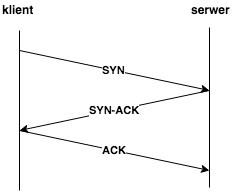
\includegraphics[height=8cm,keepaspectratio]{img/TCP_handshake.png}
    \caption{Schemat prezentujący trójstronne uzgodnienie (ang. \textit{three-way handshake}). Najpierw klient wysyła (chce zsynchronizować) swój numer sekwencji (SYN). Serwer odpowiada ACK (potwierdza udaną synchronizację) oraz SYN (synchronizacja własnego numeru sekwencji). Na końcu klient potwierdza synchronizację i może nastąpić transmisja właściwych danych.}
    \label{fig:TCP_handshake}
\end{figure}


\section{Gniazda dziedziny Uniksa}

Gniazda dziedziny Uniksa są podobne do zwykłych gniazd, jednak cała komunikacja zachodzi wewnątrz jądra systemu operacyjnego, zamiast korzystać z sieci. W tej metodzie komunikacji, system plików jest używany jako przestrzeń adresowa. Procesy traktują gniazda dziedziny Uniksa jako i-węzły (ang. \textit{i-nodes}), więc wiele procesów może komunikować się poprzez otwieranie tego samego gniazda.


\section{Systemy kolejkowe}

Systemy kolejkowe umożliwiają odłożenie wiadomości na kolejkę, z której weźmie ją odbiorca. Dzięki temu procesy nie muszą wchodzić w bezpośrednią interakcję. Cechy kolejek komunikatów zależne są od implementacji. Na przykład standard \textit{System V} posiada zarówno blokujące, jak i nieblokujące funkcje odbioru wiadomości. POSIX oferuje ponadto możliwość rejestracji funkcji odbierającej powiadomienie, która zostanie wywołana, kiedy pojawi się nowy komunikat. Dzięki temu odbiorca nie musi odpytywać kolejki (ang. \textit{polling}), marnując czas procesora, ani zatrzymywać wykonywania programu.


\section{Przekazywanie wiadomości}

Programy moga także komunikować się kanałami niezarządzanym przez system operacyjny. Wysyłana jest wiadomość, a za uruchomienie odpowiedniego kodu odpowiada odbiorca i infrastruktura wspomagająca. Ten sposób jest często używany do budowania rozproszonych aplikacji. Komunikacja może być zarówno synchroniczna, jak i asynchroniczna. Abtrakcją innego procesu może być obiekt, ale też na przykład aktor (np. stosowany w Akkce\cite{akka} model aktorów). Przesyłanie wiadomości może być zaimplementowane w dowolny sposób.


\subsection{Zdalne wykonywanie procedur}

Zdalne wykonywanie procedur (RPC - ang. \textit{remote procedure call}) to protokół utworzony przez firmę Sun\cite{rpc} i dość popularny w systemach z rodziny Unix. Służy do uruchomienia procedury w innej przestrzeni adresowej (zazwyczaj na innym komputerze w sieci). Wywołanie niczym nie różni się od lokalnych funkcji, ukrywając przed programistą szczegóły zdalnej komunikacji. Abstrakcja ta ułatwia tworzenie oprogramowania, jednak zawsze należy pamiętać, że uruchamianie kodu na innej maszynie niesie za sobą narzut komunikacyjny i nie należy go nadużywać.


\subsection{Java RMI}

Java RMI (ang. \textit{Java remote method invocation}) jest obiektowym odpowiednikiem RPC dla Javy. Technologia ta korzysta z serializacji Javy oraz rozproszonego odśmiecania pamięci (ang. \textit{distributed garbage collection}). Pozwala na zdalne wykonywanie metod na obiektach, które mogą znajdować się na innych maszynach wirtualnych Javy. Wymaganiem jest wcześniejsza rejestracja takich obiektów pod wybranymi nazwami w rejestrze \textit{RMI Registry}. Klient może pobrać tzw. \textit{stub}, czyli obiekt umożliwiający komunikację ze zdalną implementacją, mający taki sam interfejs. Wywoływanie metod jest idenetyczne jak w przypadku lokalnych obiektów. Rejestr nie pośredniczy w komunikacji. Wadą tej technologii jest brak wsparcia dla innych języków programowania.


\subsection{CORBA}

CORBA jest standardem zdefiniowanym przez OMG (ang. \textit{Object Management Group}) wydanym w 1991 roku \cite{CORBA}. Celem jest umożliwienie komunikacji między procesami stworzonymi z użyciem innych języków programowania, na niezależnych maszynach bez względu na sprzęt, czy systema operacyjny. Wykorzystany jest model obiektowy, mimo to języki programowania nie muszą wspierać paradygmatu obiektowego, aby używać technologii CORBA.

CORBA wprowadza warstwę abstrakcji, która ukrywa różnice pomiędzy systemami. Wykorzystany został język opisu interfejsu (IDL - ang. \textit{Interface Description Language}). Każdy język programowania kompiluje pliki IDL na kod zajmujący się przekazaniem metod, a w przypadku języków interpretowanych, IDL jest interpretowany w czasie wykonania. CORBA specyfikuje sposób mapowania IDL dla języków programowania takich jak np. C, C++, Java, Ada, COBOL, Lisp, Object Pascal, Python, Ruby czy Smalltalk. Zazwyczaj implementacja ORB (ang. \textit{Object Request Broker}) dostarcza kompilator IDL.


\begin{lstlisting}[caption={Przykład użycia IDL},captionpos=b]
    module ModuleExample {
        interface Math  {
            double sum(in double x, in double y);
        };
    };
\end{lstlisting}


Skorzystać możemy z wielu predefiniowanych typów (np. \textit{short}, \textit{long}, \textit{double}, \textit{string}), jak również tworzyć własne struktury czy unie oparte o typy elementarne.

W technologii CORBA istnieje jawny podział na klienty i serwery. Klient posiada interfejs pożądanego obiektu oraz jego implementację, która zostanie oddelegowana do serwera. Aby się z nim połączyć trzeba posiadać jego referencję - IOR (ang. \textit{Interoperable Object Reference}). Alternatywną jest skorzystanie z serwisu nazw (ang. \textit{NameService}) - działa on podobnie do systemu nazw domenowych (DNS). Serwer rejestruje się w nim pod wybraną nazwą, by klient mógł za jej pomocą uzyskać zarejestrowany IOR.

\begin{figure}[h]
    \centering
    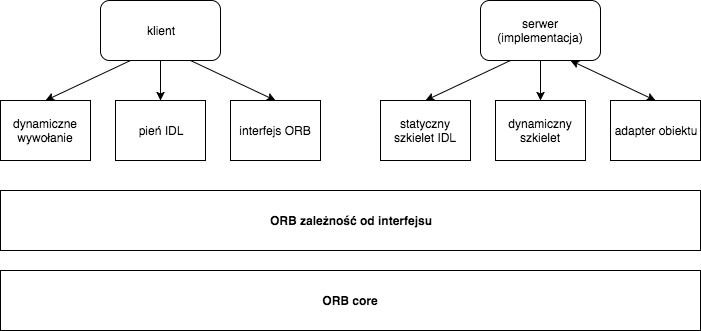
\includegraphics[width=\textwidth,height=\textheight,keepaspectratio]{img/CORBA_architecture.png}
    \caption{Schemat architektury aplikacji korzystającej z technologii CORBA \cite{Saw02}.}
    \label{fig:CORBA_architecture}
\end{figure}


\section{Java Native Interface}

Java Native Interface (JNI) co prawda nie jest metodą komunikacji między procesami, mimo to umożliwia integrację z programami napisanymi w innych językach. Pozwala, aby kod Javy uruchomiony w wirtualnej maszynie wywoływał oraz był wywoływany przez natywne aplikacje (napisane mogą one być w C, C++, asemblerze, ale także na przykład w Go i Rust) \cite{JNI17}.

Cel JNI to możliwość wykonania wszystkiego co nie jest wykonalne używając jedynie Javy, np. wykorzystywywanie bibliotek zależnych od platformy oraz zwiększenie wydajności w krytycznych obszarach aplikacji.

Natywne programy mogą korzystać z obiektów Javy (tworzyć je, wykonywać metody, odbierać przekazane w parametrach). Sama biblioteka standardowa Javy wykorzystuje tę technologię.

\begin{table}[h!]
  \centering
  \begin{tabular}{|c|c|c|}
    \hline
    \textbf{Typ w Javie} & \textbf{Typ w JNI} & \textbf{Opis} \\ [0.5ex]
    \hline
    boolean & jboolean & 8 bitów bez znaku \\
    byte & jbyte & 8 bitów ze znakiem \\
    char & jchar & 16 bitów bez znaku \\
    short & jshort & 16 bitów ze znakiem \\
    int & jint & 32 bity ze znakiem \\
    long & jlong & 64 bity ze znakiem \\
    float & jfloat & 32 bity \\
    double & jdouble & 64 bity \\
    void & void & - \\ [1ex]
    \hline
  \end{tabular}
  \caption{Mapowania typów w JNI}
\end{table}


\section{REST}

REST jest stylem architektonicznym służącym do reprezentacji zasobów oraz ich manipulacji. Korzysta on z protokołu HTTP (sekcja \ref{HTTP_section}). Nie oferuje serwisów, które można wykorzystać, lecz zasoby, na których pozwala wykonywać akcje.

Wykorzystywane są metody HTTP, które wykonują akcje zgodne ze specyfikacją \cite{RFC7231}. Zasoby adresowane są za pomocą URI. REST nie jest protokołem, brakuje więc standardu jasno go opisującego. Formatem danych najczęściej jest JSON. Metody takie jak na przykład GET, PUT, DELETE są idempotentne, to znaczy, że wielokrotne ich wywołanie powoduje identyczny efekt jak jednokrotne.

Rozwinięciem jest HATEOAS (ang. \textit{Hypermedia As The Engine Of Application State}). Odpowiedzi serwera zwierają wtedy linki do innych zasobów, umożliwiając przejście wszystkich powiązań pomiędzy obiektami przez klienta. Analogicznie działają hiperłącza zamieszczone na stronach internetowych, dzięki czemu użytkownik może się nawigować znając tylko jeden adres.

\begin{table}[h!]
  \centering
  \begin{tabular}{|c|c|c|}
    \hline
    & \textbf{Pojedynczy zasób np.} & \textbf{Kolekcja np.} \\
    & \url{http://example.com/api/items/1} & \url{http://example.com/api/items} \\ [0.5ex]
    \hline
    \textbf{GET} & Zwraca reprezentację zasobu & Zwraca całą kolekcję \\
    \hline
    \textbf{POST} & \begin{tabular}{@{}c@{}} Tworzy nowy zasób wykorzystując wysłany \\ przez klienta, zazwyczaj w odpowiedzi \\ znajduje się adres nowego elementu \end{tabular} &  Zazwyczaj nie używany \\
    \hline
    \textbf{PUT} & \begin{tabular}{@{}c@{}} Zamienia wybrany zasób \\ na wysłany przez klienta \end{tabular} & \begin{tabular}{@{}c@{}} Zamienia całą kolekcję \\ na wysłaną przez klienta \end{tabular} \\
    \hline
    \textbf{DELETE} & Usuwa zasób & Usuwa całą kolekcję \\
    \hline
  \end{tabular}
  \caption{Sposób działania przykładowych metod HTTP na zasobach}
\end{table}


\subsection{Protokół HTTP}

\label{HTTP_section}
HTTP (ang. \textit{Hypertext Transfer Protocol}) to bezstanowy protokół przesyłania dokumentów hipertekstowych w sieci WWW (ang. \textit{World Wide Web}). Do transportu wykorzystuje TCP. Jego działanie określić można jako zapytanie-odpowiedź. Klientem może być przeglądarka internetowa, która dokonuje żądań zasobów. Żądania te składają się z metody (np. GET, POST, HEAD, PUT, DELETE, OPTIONS) oraz Ujednoliconego Identyfikatora Zasobów (URI - ang. \textit{Uniform Resource Identifier}). W zapytaniu wysłane mogą być nagłówki (np. Accept, Content-Type, Host, Authorization). Metody takie jak POST, PUT umożliwiają wysłanie ciała zapytania (np. wiadomość w formacie JSON, XML). Odpowiedź od serwera także zawiera nagłówki i ciało, ale również kod statusu, który dostarcza dodatkowych informacji:
\begin{itemize}
  \item 1xx - kody informacyjne
  \item 2xx - kody powodzenia
  \item 3xx - kody przekierowania
  \item 4xx - kody błędu aplikacji klienta
  \item 5xx - kody błędu serwera HTTP
\end{itemize}


\begin{lstlisting}[caption={Przykład żądania HTTP},captionpos=b]
    GET /index.html HTTP/1.1
    Host: www.example.com
\end{lstlisting}

Serwer zwraca odpowiedź lub informuje o wystąpieniu błędu:

\begin{lstlisting}[caption={Przykład odpowiedzi serwera ze statusem 200 OK},captionpos=b]
    HTTP/1.1 200 OK
    Date: Mon, 11 May 2017 21:17:46 GMT
    Content-Type: text/html; charset=UTF-8
    Content-Encoding: UTF-8
    Content-Length: 138
    Last-Modified: Wed, 08 Jan 2003 23:11:55 GMT
    Server: Apache/1.3.3.7 (Unix) (Red-Hat/Linux)
    Connection: close

    <html>
        <head>
            <title>Przykładowy tytuł</title>
        </head>
        <body>
            Przykładowa odpowiedź
        </body>
    </html>
\end{lstlisting}


\section{Porównanie wydajności potoków, pamięci współdzielonej oraz gniazda dziedziny Uniksa}

Porównując niskopoziomowe rozwiązania, ściśle powiązane z systemem operacyjnym dostrzec można pewną zależność \cite{ZX2011}:

\begin{itemize}
    \item dla danych mniejszych niż 4600 bajtów - pamięć współdzielona jest najszybsza
    \item dla danych między 5100 a 12000 bajtów - gniazdy dziedziny Uniksa okazały się najlepsze
    \item w pozostałych przypadkach zwyciężyły potoki nienazwane
\end{itemize}
